\problemname{}

%\illustration{0.3}{image.jpg}{
%    Caption of the illustration (optional).
%    CC BY-SA 4.0 by X on \href{https://example.com/reference-to-image}{Y}
%}

% optionally define variables/limits for this problem
\newcommand{\maxk}{10^9}
\newcommand{\wa}{A}
\newcommand{\wb}{B}
\newcommand{\wc}{C}

\illustration{0.3}{hanging}{Laundry hanging to dry \\\href{https://pixabay.com/photos/hanging-architecture-clothesline-3282769/}{Image by gregroose on Pixabay}}%
Every Sunday is laundry day, and there is always a huge pile of clothes waiting to be washed, which is certainly going to take you forever. 
You are particularly annoyed by how careful you have to be when washing certain items, and how important it is that you choose an appropriate washing programme for each item. 

Fortunately, your washing machine is quite old and only supports three different washing programmes: \wa, \wb, and \wc.
You can put at most $k$ items in one load, 
and each load can be washed using one of the programmes. 

Some items are easy to care for, and you can put them in any load you like. 
More delicate items must not be washed using a specific programme, but the other two are fine. 
Of course, the worst clothes are the ones for which only one programme is appropriate. 

You have already sorted the items into seven piles by putting items together for which the same combination of programmes is fine, so 
you know how many items are in each pile. 

What is the minimum number of loads you need to wash? 

\begin{figure}[!h]
	\centering
	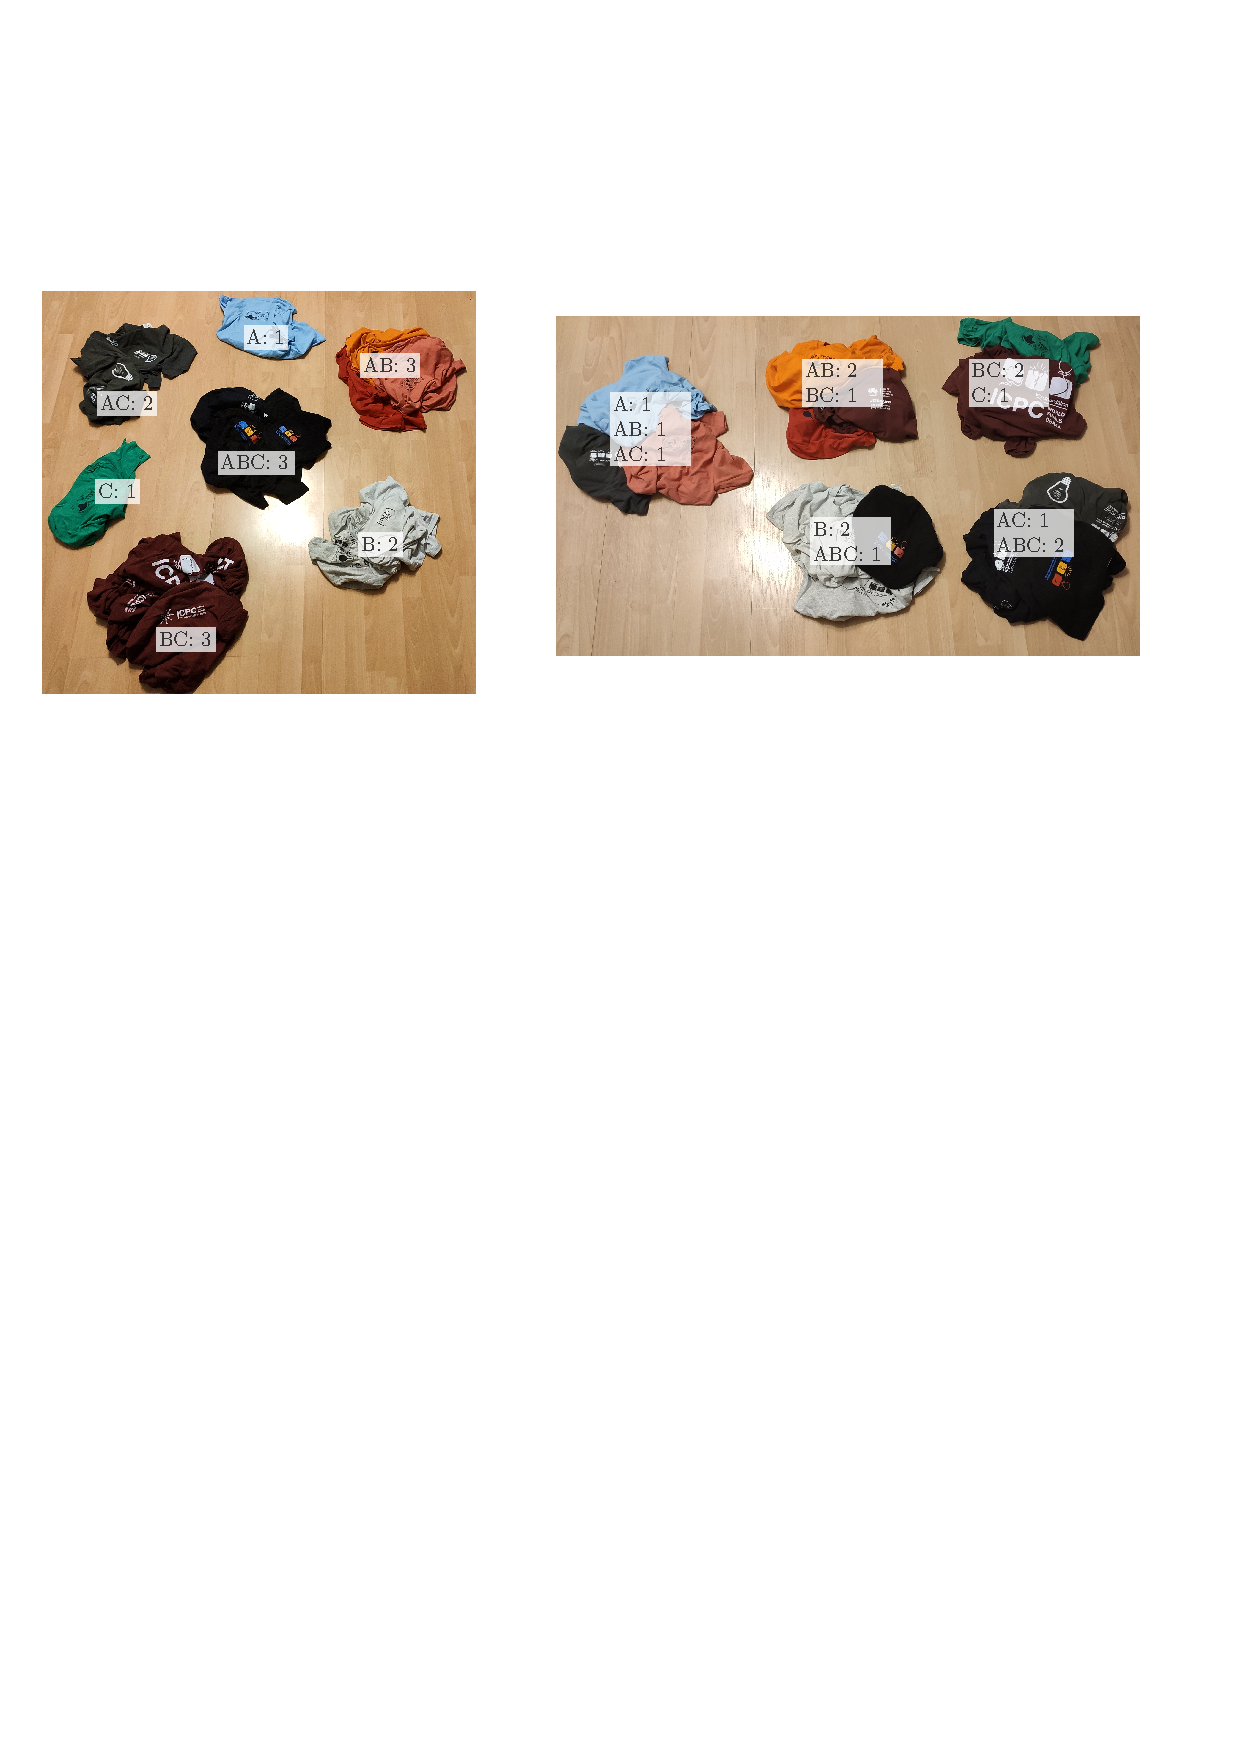
\includegraphics[width=0.9\textwidth]{sample_2}
	\caption{Illustration of Sample Input 2 with an optimal solution.
    The figure on the left shows seven piles, one for each combination. 
    The figure on the right shows a (possible) optimal solution, where each pile is washed in one load.
    The numbers on the pile represent how many items of each combination are washed with this load. 
    In particular, the leftmost pile is washed using programme A, the two piles in the middle with programme B, and the two piles on the right with programme C. 
    Thus, we need five loads to wash all items, which is optimal since we have $15$ items in total.  
    % The number after each combination denotes how many items are in each pile.  
    % The numbers on the arrows represent how many items of some combination is assigned a certain washing programme for this particular solution. 
    % For example, for combination $AB$, one item is washed using programme $A$, and two items are washed using programme $B$.
    % In total, we have three items for $A$, six items for $B$, and six items for $C$. 
    % Since $k$ is $3$, we need five loads to wash all items. 
    % This is optimal, as we have 15 items in total.   
    }
\end{figure}

\begin{Input}
    The input starts with a line containing one integer $t$ ($1 \leq t \leq 10^4$), the number of test cases.
    Then for each test case: 
    \begin{itemize}
        \item One line with an integer $k$ ($1\leq k\leq \maxk$), the number of items you can put in one load.
        \item One line with seven integers $c_1, \ldots, c_7$ ($0 \leq c_i \leq \maxk$), the number of items for each combination of programmes. 
        The integers are given in this order: \wa, \wb, \wc, \wa\wb, \wb\wc, \wa\wc, \wa\wb\wc. 
        For example, $c_4$ must be washed using either programme \wa{} or programme \wb.  
    \end{itemize}
\end{Input}

\begin{Output}
    For each test case, output the minimum number of loads that are needed to wash all clothes. 
\end{Output}
